\documentclass[11pt,a4paper]{article}
\usepackage[T1]{fontenc}
\usepackage[utf8]{inputenc}
\usepackage{lmodern}
\usepackage[a4paper,left=2.6cm,right=2.6cm,top=2.8cm,bottom=2.8cm]{geometry}
\usepackage{amsmath,amssymb,amsthm}
\usepackage{booktabs,graphicx,microtype,xcolor,fancyhdr,caption,enumitem,float}
\usepackage[hidelinks]{hyperref}
\captionsetup{font=small,labelfont=bf}
\captionsetup[table]{position=above,skip=4pt}
\setlist{itemsep=2pt,topsep=4pt}
\theoremstyle{definition}
\newtheorem{definition}{Definition}[section]
\newtheorem{result}{Result}[section]
\theoremstyle{remark}
\newtheorem{remark}{Remark}[section]
\pagestyle{fancy}\fancyhf{}
\fancyfoot[L]{\footnotesize Théo Lacoste $\cdot$ \texttt{github.com/lacostetheo/ML-PREDICTION-OLYMPIQUE-LYONNAIS}}
\fancyfoot[R]{\footnotesize\thepage}
\renewcommand{\headrulewidth}{0pt}
\setlength{\parindent}{0pt}\setlength{\parskip}{5pt}
\usepackage{titlesec}
\titleformat{\section}{\large\bfseries}{\thesection}{1em}{}
\titleformat{\subsection}{\normalsize\bfseries}{\thesubsection}{1em}{}
\titlespacing*{\section}{0pt}{16pt}{6pt}
\titlespacing*{\subsection}{0pt}{10pt}{4pt}
\newcommand{\E}{\mathbb{E}}
\begin{document}

\thispagestyle{fancy}
\begin{center}
{\Large\bfseries Machine Learning Project: Predicting the Victories\\[2pt] of Olympique Lyonnais}\\[10pt]
{\large\bfseries Walk-Forward Validation, Probabilistic Forecasts,\\[1pt] Monte Carlo Season Simulation, and a Test Against the Betting Market}\\[16pt]
{\large Théo Lacoste}\\[2pt]
{\small EDHEC Business School}\\[2pt]
{\small \texttt{github.com/lacostetheo/ML-PREDICTION-OLYMPIQUE-LYONNAIS}}\\[10pt]
{\normalsize October 27, 2026}
\end{center}
\vspace{2pt}
\begin{center}\begin{minipage}{0.88\textwidth}\small\itshape
\textbf{Disclaimer.} I hope the ML does not predict well, because what the f***, OL will be 5th this season.
(The simulation puts the average final position of OL at 5.9. So much for my hopes.)\ \ Joke aside, let us begin.
\end{minipage}\end{center}
\vspace{6pt}
\begin{center}\textbf{Abstract}\end{center}
\vspace{-4pt}
\begin{center}\begin{minipage}{0.88\textwidth}\small
This project was carried out in October 2026, two months into the 2026/27 season, and every ``current'' number refers to the state of 27 October 2026 (8 Ligue 1 matches played).
We ask whether machine learning can forecast the results of Olympique Lyonnais (OL) better than an Elo rating or the betting market.
On 29{,}287 matches of the five major European leagues (2010/11 to October 2026) we build features strictly from information available before kick-off, checked by an automated perturbation test,
and compare Elo, Poisson, logistic regression, random forest, gradient boosting, SVM and neural networks on a walk-forward test of 5{,}650 matches.
(i)~The \emph{chosen model} is a multinomial logistic regression on 100 variables, refitted every season.
(ii)~Boosting and neural networks are statistically indistinguishable from it (log loss 0.979); all beat Elo (0.989) but none beats the bookmaker (0.966).
(iii)~Pooling our probabilities with the market's adds nothing: the optimal weight on the model is zero.
(iv)~Elo and squad market value explain almost everything that is predictable.
A Monte Carlo simulator, backtested on 2023--2025, projects OL at 54.6 points (80\% interval 46--63), an average final position of 5.9 and a 36\% chance of the top four.
The Champions League and the Europa League, which OL plays this season, have no clear favourite: the best-placed club wins only 14\% and 15\% of the simulations respectively.
\end{minipage}\end{center}
\section{Introduction}

\textbf{When this was done.} This project was carried out in \textbf{October 2026}, two months into the 2026/27 season. Eight rounds of Ligue 1 had been played; the data end with the matches of 26 October 2026,
and the snapshot used for all forecasts is dated 27 October 2026. Anything described as ``current'', ``next'' or ``projected'' refers to that date and will change as the season goes on.

Football is the sport where the gap between a simple forecast and the best one is smallest: a match is decided by a handful of goals,
the stronger team wins only about one time in two, and one game in four ends in a draw. This makes it a good laboratory for a question that also matters in finance:
\emph{how much can a model extract from public data, how reliably can that be measured, and does it survive comparison with a liquid market?}

OL plays about 35 league matches a year, far too few to train a model. I therefore train on all five major leagues (Premier League, La Liga, Serie A, Bundesliga, Ligue 1)
and use OL as a case study. The object to forecast is the following.

\begin{definition}[Match forecast]
A \emph{match forecast} is a probability vector $p=(p_A,p_D,p_H)$ over the outcomes away win, draw and home win, computed from information available before kick-off.
The \emph{expected points} of the home side are $3p_H+p_D$.
\end{definition}

For instance, for OL's next Ligue 1 match, Lyon--Angers on Saturday 31 October 2026, the model gives the forecast of Table~\ref{tab:next}.

\begin{table}[H]
\caption{Forecast for Lyon--Angers (Ligue 1, Saturday 31 October 2026).\label{tab:next}}
\begin{center}
\small
\begin{tabular}{lcccc}
\toprule
\textbf{} & \textbf{OL win} & \textbf{Draw} & \textbf{OL loss} & \textbf{OL expected points} \\
\midrule
Model & 68\% & 20\% & 12\% & 2.23 \\
\bottomrule
\end{tabular}
\end{center}
\end{table}

\textbf{The model I chose.} A \emph{multinomial logistic regression} on 100 input variables (Elo rating, squad market value, recent form, shots, schedule),
refitted once a year (Section~\ref{sec:model}). I also tested random forest, gradient boosting, a support-vector machine and neural networks, all with scikit-learn.
None is significantly better, so I kept the simplest and most explainable one.

\textbf{Three rules.} (1)~\emph{No leakage}: a variable used to predict a match played at date $T$ contains nothing dated $T$ or later.
(2)~\emph{Temporal validation}: train on the past, judge on the future, never on a random split.
(3)~\emph{Honest evidence}: every claimed improvement comes with a confidence interval, and negative results are reported as negative.

\section{Data}

\begin{table}[H]
\caption{Data sources.}
\begin{center}
\small
\begin{tabular}{p{3.6cm}p{8.2cm}l}
\toprule
\textbf{Source} & \textbf{Content} & \textbf{Use} \\
\midrule
football-data.co.uk & Results, shots, corners, cards, bookmaker odds; 5 leagues, 2010/11--2026 & Core data \\
Transfermarkt dataset (CC0) & 656{,}000 player market valuations & Squad value \\
Self-computed & Elo ratings, shot-based ``xG proxy'' & Variables \\
Wikipedia & Champions League and Europa League 2026/27 fixtures and scores & Section~\ref{sec:ucl} \\
openfootball, Maxifoot & Calendars of the matches still to play (dates only) & Display \\
\bottomrule
\end{tabular}
\end{center}
\end{table}

The sample has 29{,}287 matches (594 for OL) and 189 clubs: training 2011--2020 (about 18{,}200 matches), validation 2021--22 (3{,}651) and test October 2023 to October 2026 (5{,}650).
\textbf{Rejected sources.} FBref advanced statistics were removed by their provider in January 2026; Understat forbids automated access in its \texttt{robots.txt}; ClubElo was unreachable.
No free historical source exists for injuries or line-ups, so they could not be tested.
\textbf{Terms of use.} football-data.co.uk allows private, non-commercial use only. This is a private academic study: raw data are downloaded, kept out of the repository and not redistributed.

\section{Variables and leakage control}

Every variable is computed for the home team, the away team and their difference, from matches strictly before the one predicted.

\begin{definition}[Leakage-free variable]
A variable attached to a match played at date $T$ is \emph{leakage-free} if it is a function of results dated strictly before $T$ only.
\end{definition}

\begin{table}[H]
\caption{Families of variables.}
\begin{center}
\small
\begin{tabular}{p{3.0cm}p{9.5cm}}
\toprule
\textbf{Family} & \textbf{Construction} \\
\midrule
Elo rating & Strength score updated after every match (below), one scale per league \\
Recent form & Mean over the last 3, 5, 10 matches of points, goals for and against, shots on target \\
Venue form & Last 5 home (or away) matches \\
League table & Points and goal difference per match, position before the match \\
Schedule & Rest days, matches in the previous 14 days \\
Squad value & $\ln V$ of the team minus the league average of that month (Transfermarkt) \\
\bottomrule
\end{tabular}
\end{center}
\end{table}

\textbf{Elo} \cite{elo1978}\textbf{.} Before a match between $i$ (home) and $j$ (away), the expected score of the home team is
\begin{equation}E_{ij}=\frac{1}{1+10^{-(R_i-R_j+65)/400}},\end{equation}
where 65 points is the home advantage. With $S=1$, $\tfrac12$, $0$ for a win, draw, loss and $g$ the goal difference, the ratings are updated after the match by
\begin{equation}R_i' = R_i + K\,\bigl(1+\ln(1+|g|)\bigr)\,(S-E_{ij}),\qquad R_j' = R_j - (R_i'-R_i),\qquad K=20.\end{equation}
The rating stored for the match is the one \emph{before} this update.

\textbf{Squad value} is measured relative to the league so that market inflation is not mistaken for strength:
\begin{equation}sv_i=\ln V_i-\frac{1}{|L|}\sum_{k\in L}\ln V_k.\end{equation}

\textbf{How leakage is prevented.} Rolling variables are shifted by one match; Elo is stored before its update; valuations used for the squad value are dated before the monthly snapshot;
bookmaker odds are never a variable. An automated test replaces every result after a cutoff date by random values, reruns the whole pipeline and requires all earlier variables to be identical.
It fails, as it should, on two bugs I injected on purpose (a rolling window without the shift, Elo stored after its update).

\textbf{Two lessons from the data.} The ``xG proxy'' (a regression of goals on shots) collapses to $0.287\times$ shots on target, so it is not a real xG.
Variables counting how many matches a team has been observed for are just a calendar clock; I removed them (cost $+0.0011$ log loss on validation, not significant).

\section{The model I chose: multinomial logistic regression}\label{sec:model}

\begin{definition}[Multinomial logistic regression]
Let $x\in\mathbb{R}^{100}$ be the (standardised) variables of a match. For each outcome $k\in\{A,D,H\}$ the model computes a linear score $z_k=w_k^\top x+b_k$ and returns
\begin{equation}P(\text{outcome}=k\mid x)=\frac{\exp(w_k^\top x+b_k)}{\sum_{j\in\{A,D,H\}}\exp(w_j^\top x+b_j)}.\end{equation}
\end{definition}

\textbf{Estimation.} The weights maximise the log-likelihood of the training matches, with an $L^2$ penalty that keeps them small:
\begin{equation}\min_{W,b}\; -\frac1N\sum_{i=1}^{N}\ln P(y_i\mid x_i)\;+\;\frac{1}{2CN}\,\|W\|^2 .\end{equation}
The strength $1/C$ of the penalty is chosen by \emph{time-ordered} cross-validation inside the training seasons (each fold trains on the past and scores the next block).
Variables are standardised and missing values replaced by the median, both fitted on training data only. The model is refitted once a year.

\begin{remark}[Why this model]
(a) It is as accurate as the alternatives (Section~\ref{sec:results}). (b) It is explainable: the linear scores split exactly into the contribution of each family of variables,
$z_k=b_k+\sum_f c_{k,f}$, which the website displays. (c) Its probabilities are well calibrated. (d) It is fast enough to simulate 10{,}000 seasons per league.
\end{remark}

\begin{table}[H]
\caption{Models compared.}
\begin{center}
\small
\begin{tabular}{p{3.0cm}p{9.5cm}}
\toprule
\textbf{Family} & \textbf{Models compared} \\
\midrule
Baselines & Class frequencies; league table; Elo calibrated to 3 classes; independent Poisson goals \cite{dixon1997} \\
Linear (chosen) & Multinomial logistic regression with $L^2$ penalty \\
Trees & Random forest; gradient boosting \\
Kernel & RBF support-vector machine (under-tuned) \\
Neural & MLP with 1 and 2--3 hidden layers ($L^2$, few epochs, mean of 5 seeds) \\
Online & Logistic regression whose weights are updated by gradient descent after each week of results \\
Reference & Bet365 prices turned into probabilities (margin removed, average margin 5.5\%) \\
\bottomrule
\end{tabular}
\end{center}
\end{table}

Only scikit-learn \cite{pedregosa2011} and numpy are used. Dropout and Batch Normalisation do not exist in scikit-learn; I replaced them by an $L^2$ penalty, few epochs and seed averaging.
LSTM and GRU networks were not built: the rolling variables already summarise each team's history.

\section{How quality is measured}

Accuracy is a weak summary here: a draw is almost never the most likely outcome, so a useful model can rarely name one. The main metric is the log loss, a strictly proper scoring rule \cite{gneiting2007}.

\begin{definition}[Log loss]
For $N$ matches, with $p_i$ the probability given to the outcome that actually occurred in match $i$,
\begin{equation}\mathrm{LL}=-\frac1N\sum_{i=1}^{N}\ln p_i .\end{equation}
\end{definition}

\emph{Example.} If the model gave 20\% to what happened, the match costs $\ln 5=1.61$; if it gave 60\%, it costs $0.51$.
A model that always says $(30.0\%,25.2\%,44.7\%)$ (the average frequencies) scores $1.075$; a model that knew the result would score $0$.

I also report the Brier score \cite{brier1950} and the expected calibration error:
\begin{equation}\mathrm{Brier}=\frac1N\sum_{i=1}^{N}\sum_{k}(p_{ik}-o_{ik})^2,\qquad \mathrm{ECE}=\sum_{b}\frac{n_b}{N}\,\bigl|\bar p_b-\bar o_b\bigr|,\end{equation}
where $o_{ik}=1$ if outcome $k$ occurred in match $i$ and $0$ otherwise, and $b$ indexes bins of forecast probabilities.

\textbf{Significance.} To compare models $A$ and $B$, I take the paired difference $\Delta=\overline{\ell_A-\ell_B}$ of their per-match log losses and build a 95\% confidence interval by a \emph{block bootstrap}
that resamples whole calendar weeks (matches of the same week are not independent), with 4{,}000 draws. With 5{,}600 test matches, a difference below about 0.003 cannot be detected.

\section{Validation design}

Football results form a time series: a random split would let the model learn from matches played after those it is tested on.
Training covers 2011--2020, validation 2021--22 (used to compare models during development) and test October 2023 to October 2026 (used once, with frozen hyper-parameters).
The final evaluation is \emph{walk-forward}: each test season $S$ is predicted by models fitted on seasons $2011,\dots,S-1$, as it would run in real life.

\section{Results}\label{sec:results}

\begin{table}[H]
\caption{Walk-forward test, October 2023 to October 2026 (5{,}650 matches).}
\begin{center}
\small
\begin{tabular}{lcccc}
\toprule
\textbf{Model} & \textbf{Accuracy} & \textbf{Log loss [95\% CI]} & \textbf{Brier} & \textbf{ECE} \\
\midrule
Baseline (frequencies) & 43.2\% & 1.0754 [1.069, 1.082] & 0.6509 & 0.012 \\
Elo & 52.5\% & 0.9892 [0.979, 0.999] & 0.5902 & 0.017 \\
Poisson goals & 52.0\% & 0.9907 [0.980, 1.001] & 0.5908 & 0.022 \\
\textbf{Logistic regression (chosen)} & \textbf{53.2\%} & \textbf{0.9794 [0.969, 0.990]} & \textbf{0.5835} & \textbf{0.017} \\
Gradient boosting & 52.9\% & 0.9787 [0.968, 0.989] & 0.5826 & 0.020 \\
Neural network (MLP) & 52.9\% & 0.9799 [0.970, 0.990] & 0.5836 & 0.021 \\
Ensemble of the three & 53.0\% & 0.9781 [0.968, 0.988] & 0.5825 & 0.017 \\
Bookmaker (Bet365) & 53.9\% & 0.9659 [0.956, 0.976] & 0.5741 & 0.022 \\
\bottomrule
\end{tabular}
\end{center}
\end{table}

\begin{figure}[H]\centering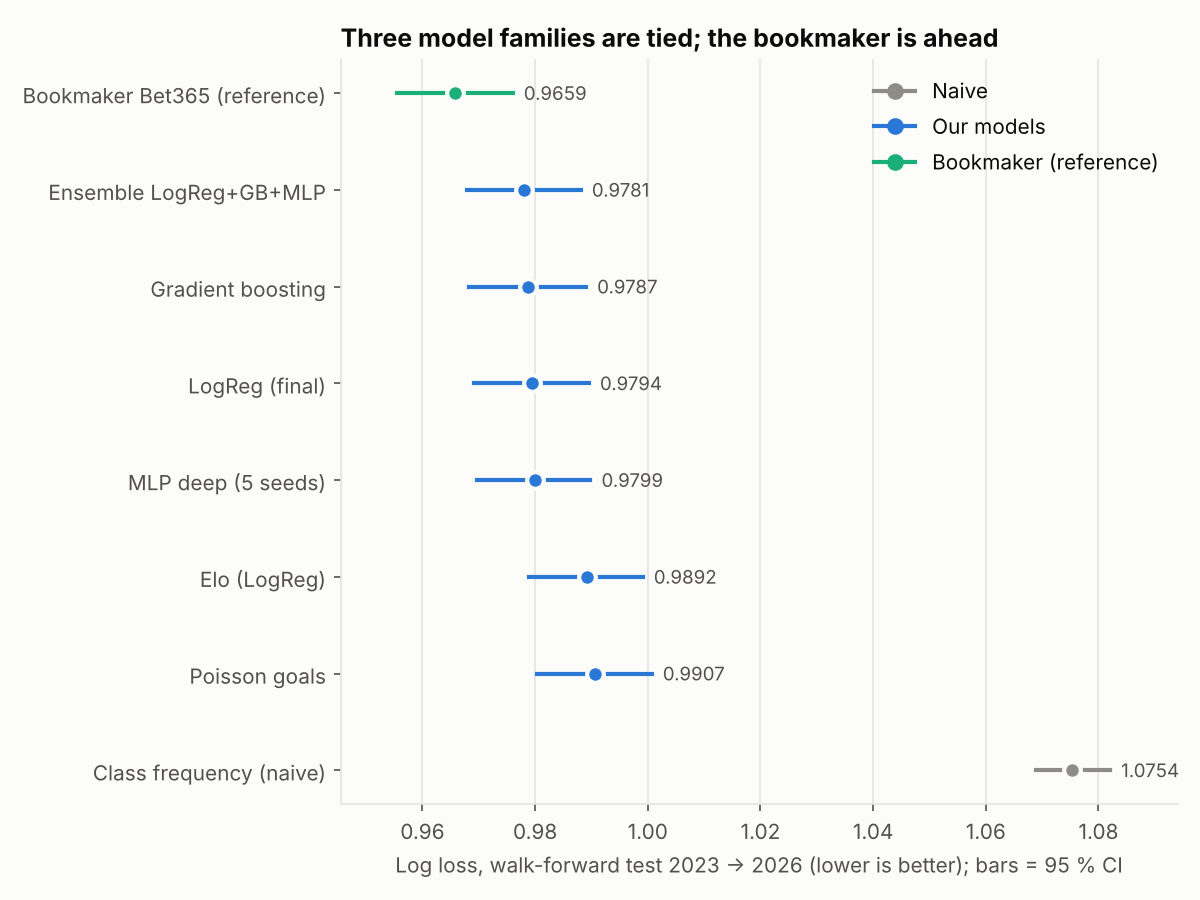
\includegraphics[width=0.8\textwidth]{figures/final_logloss.png}\caption{Log loss on the test seasons with 95\% confidence intervals: three model families are tied, the bookmaker is ahead.}\label{fig:ll}\end{figure}

\begin{result}
The logistic regression beats Elo ($\Delta=-0.0098$, 95\% CI $[-0.0137,-0.0060]$). Gradient boosting ($-0.0007$) and the neural network ($+0.0005$) do \emph{not} beat it: their intervals contain 0.
The bookmaker beats every model ($\Delta=+0.0136$ for the logistic regression, CI $[+0.0093,+0.0178]$). Complexity did not pay.
\end{result}

\subsection{Calibration}

\begin{figure}[H]\centering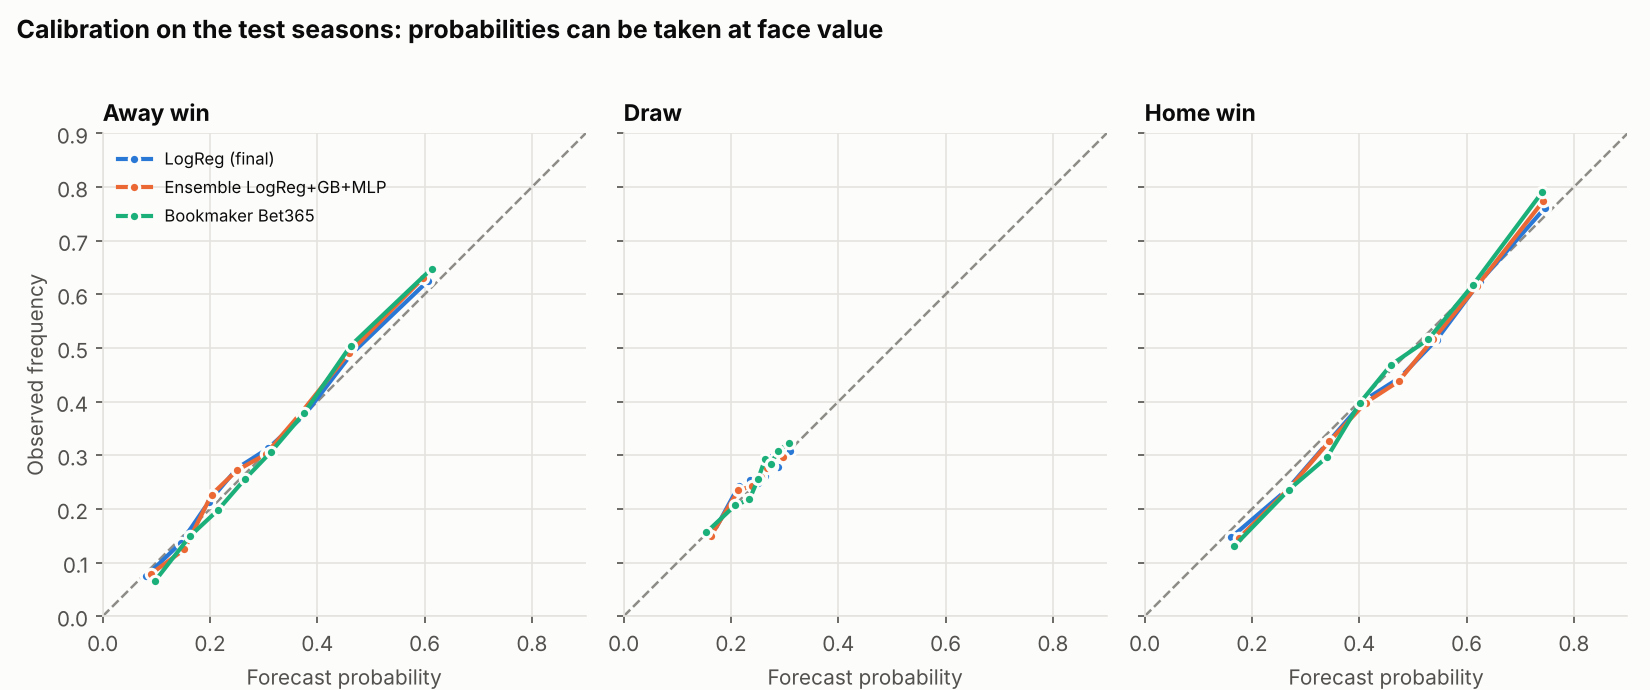
\includegraphics[width=0.95\textwidth]{figures/final_reliability.png}\caption{Reliability diagrams on the test seasons: the closer to the diagonal, the more honest the forecast.}\label{fig:rel}\end{figure}

The probabilities are well calibrated (ECE between 1.7\% and 2.2\%). The model almost never names a draw as the most likely outcome (6 matches out of 5{,}650): draws are essentially unpredictable.

\subsection{Ablation: which data add value?}

\begin{table}[H]
\caption{Ablation: nested blocks of variables (validation seasons).}
\begin{center}
\small
\begin{tabular}{lcc}
\toprule
\textbf{Logistic regression, validation} & \textbf{Log loss} & \textbf{Change vs previous [95\% CI]} \\
\midrule
A: Elo only & 0.9957 & -- \\
B: + results form & 0.9931 & $-0.0026$ $[-0.0051,-0.0001]$ \\
C: + shots and xG proxy & 0.9887 & $-0.0044$ $[-0.0072,-0.0017]$ \\
D: + league table, fatigue & 0.9890 & $+0.0003$ $[-0.0013,+0.0019]$ (nothing) \\
E: + squad value (final) & 0.9870 & $-0.0020$ $[-0.0048,+0.0009]$ \\
\bottomrule
\end{tabular}
\end{center}
\end{table}

Form and shots each add a small but detectable gain on top of Elo; league position and fatigue add nothing. Squad value is not significant on two validation seasons although it ranks second in the importance analysis below:
it overlaps with Elo, both measuring long-run strength.

\section{What drives the predictions?}

\begin{figure}[H]\centering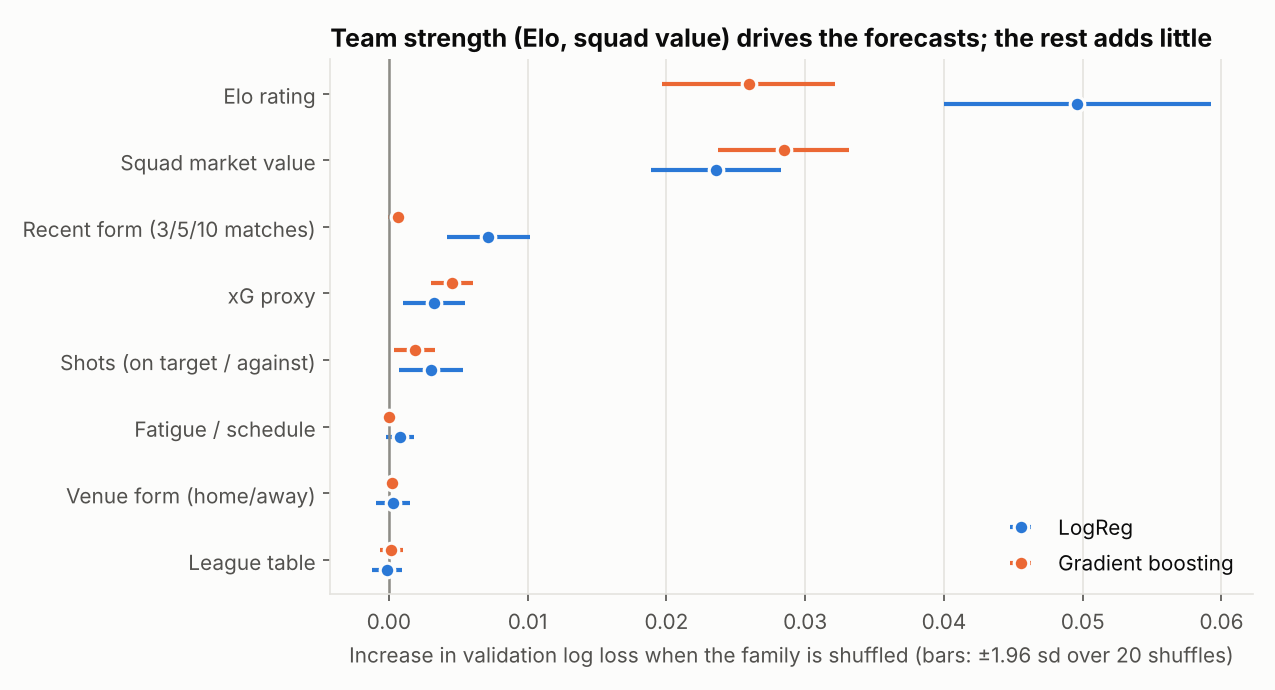
\includegraphics[width=0.78\textwidth]{figures/phase7_family_importance.png}\caption{Increase of the validation log loss when a family of variables is shuffled (permutation importance).}\label{fig:imp}\end{figure}

Elo ($+0.050$) and squad value ($+0.024$) dominate. Recent form adds $+0.007$ and shots $+0.003$; rest days, league table and venue form are close to zero.
Home sides win 44.7\% of matches, draw 25.2\% and lose 30.0\%, which sits in the intercept.

\begin{remark}
In the linear model, form has a slightly negative effect at fixed Elo and squad value. This is a collinearity artefact (overlapping windows), not evidence that a good run hurts.
Importance describes what the \emph{model} uses, not what causes results.
\end{remark}

\section{Model versus bookmaker}

This is an academic question only; no betting strategy is built. To test whether the model contains information the market lacks, I pool the two by log-linear pooling,
\begin{equation}p\;\propto\;p_{\text{market}}^{\,1-w}\;p_{\text{model}}^{\,w},\end{equation}
and choose the weight $w$ on validation. On the test seasons the best weight on the model is $w=0.00$: the market already contains everything the model knows.
The pooled log loss (0.9664) is not better than the market alone (0.9659). The market takes a margin of 5.5\% on average and is still sharper than the model; the likely reason is information I do not have (line-ups, injuries, news).

\section{Previous results: was the model right?}

\begin{remark}
These forecasts are recomputed \emph{after the fact} with the walk-forward method (models fitted only on earlier seasons, variables built only from earlier matches).
They were \textbf{not published in advance}. ``Right'' means that the most likely outcome occurred: a 45\% pick is wrong more often than right, by design, so log loss and calibration are the fair scores.
\end{remark}

\begin{table}[H]
\caption{Accuracy and log loss (LL) over recent periods.}
\begin{center}
\small
\begin{tabular}{lccccc}
\toprule
\textbf{Period} & \textbf{Matches} & \textbf{Correct} & \textbf{LL model} & \textbf{LL bookmaker} & \textbf{LL no-skill} \\
\midrule
Last 7 days (20 Oct--26 Oct 2026) & 49 & 45\% & 0.992 & 0.975 & 1.070 \\
Last 30 days (27 Sep--26 Oct 2026) & 144 & 53\% & 0.949 & 0.927 & 1.053 \\
Whole test period (2023 → Oct 2026) & 5650 & 53\% & 0.979 & 0.966 & 1.075 \\
\bottomrule
\end{tabular}
\end{center}
\end{table}

\begin{table}[H]
\caption{When the model said $x$\%, how often did it happen? (all 5{,}650 test matches)}
\begin{center}
\small
\begin{tabular}{cccc}
\toprule
\textbf{Top pick given} & \textbf{Matches} & \textbf{Mean forecast} & \textbf{Came true} \\
\midrule
0--40\% & 807 & 38\% & 39\% \\
40--50\% & 1805 & 45\% & 44\% \\
50--60\% & 1455 & 55\% & 55\% \\
60--70\% & 968 & 65\% & 64\% \\
70--100\% & 615 & 76\% & 78\% \\
\bottomrule
\end{tabular}
\end{center}
\end{table}

When the top pick was given 60--70\%, it happened 64\% of the time. Over the last 30 days of the data (27 September to 26 October 2026) the model is right 53\% of the time and is slightly less sharp than the bookmaker.

\begin{table}[H]
\caption{The 14 most recent matches before the snapshot, 2026 season (probabilities in \%).}
\begin{center}
\footnotesize
\begin{tabular}{llcccl}
\toprule
\textbf{Date} & \textbf{Match} & \textbf{Score} & \textbf{H / D / A} & \textbf{Top pick} & \textbf{Result} \\
\midrule
26 Oct & Sevilla -- Osasuna & 2--0 & 45 / 28 / 28 & Home win 45\% & Right \\
26 Oct & Paris SG -- Lyon & 2--0 & 63 / 21 / 16 & Home win 63\% & Right \\
25 Oct & Sociedad -- Levante & 2--1 & 52 / 25 / 23 & Home win 52\% & Right \\
25 Oct & Celta -- Betis & 0--0 & 39 / 24 / 36 & Home win 39\% & Wrong \\
25 Oct & Barcelona -- Real Madrid & 1--2 & 64 / 17 / 19 & Home win 64\% & Wrong \\
25 Oct & Ath Bilbao -- Getafe & 4--0 & 59 / 24 / 16 & Home win 59\% & Right \\
25 Oct & Udinese -- Milan & 0--2 & 23 / 25 / 51 & Away win 51\% & Right \\
25 Oct & Lecce -- Juventus & 0--2 & 19 / 26 / 55 & Away win 55\% & Right \\
25 Oct & Inter -- Fiorentina & 2--1 & 76 / 16 / 8 & Home win 76\% & Right \\
25 Oct & Genoa -- Venezia & 1--0 & 59 / 27 / 14 & Home win 59\% & Right \\
25 Oct & Atalanta -- Frosinone & 4--4 & 53 / 28 / 19 & Home win 53\% & Wrong \\
25 Oct & Toulouse -- Troyes & 0--0 & 62 / 24 / 14 & Home win 62\% & Wrong \\
25 Oct & Rennes -- Strasbourg & 3--0 & 50 / 24 / 26 & Home win 50\% & Right \\
25 Oct & Monaco -- Lille & 1--1 & 44 / 26 / 30 & Home win 44\% & Wrong \\
\bottomrule
\end{tabular}
\end{center}
\end{table}

\section{Case study: Olympique Lyonnais}

\begin{figure}[H]\centering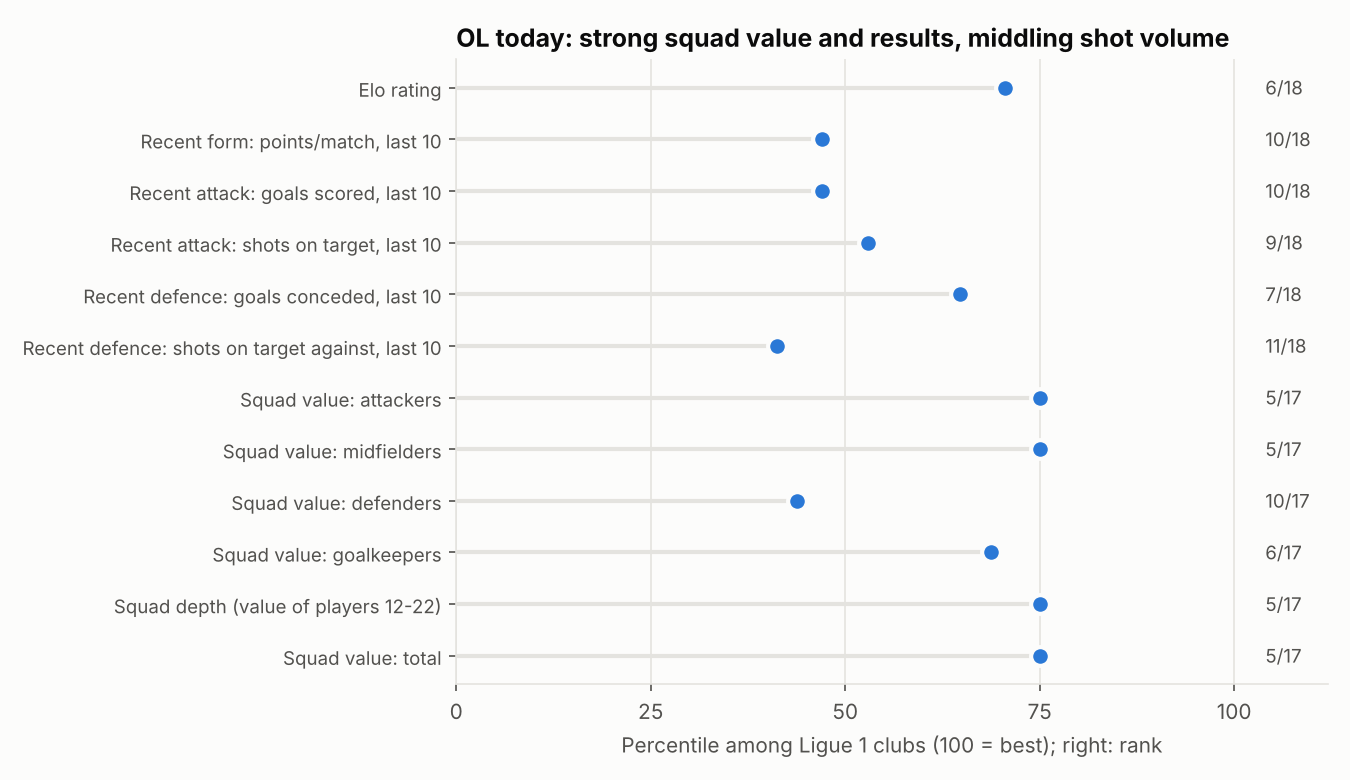
\includegraphics[width=0.8\textwidth]{figures/ol_strength_profile.png}\caption{OL's profile in Ligue 1 on 27 October 2026 (percentile among clubs; right: rank).}\label{fig:prof}\end{figure}

OL is sixth in Ligue 1 by Elo (1{,}602; Paris SG 1{,}719), tenth for recent points and tenth for goals scored,
and fifth by squad value (EUR 305 m; the defence is tenth). Its shot volume (shots on target) ranks ninth.
For Lyon--Angers, the 90\% interval on OL's win probability is 62--73\% once model uncertainty (100 bootstrap refits) and uncertainty on the true strength of both teams (Elo shaken by 60 points) are added.

\section{Season simulation}

\begin{definition}[Simulated season]
Given the current state, a \emph{simulated season} (i)~shakes the Elo rating of every team by $\varepsilon\sim\mathcal{N}(0,60^2)$, (ii)~draws the outcome of each remaining match from the model's probabilities,
(iii)~draws a scoreline from a Poisson goal model consistent with that outcome (for goal-difference tie-breaks) and (iv)~ranks the table on points, goal difference and goals scored.
The expected points of a team are its current points plus $\sum_{m}(3p^{(m)}_{\mathrm{win}}+p^{(m)}_{\mathrm{draw}})$ over its remaining matches.
\end{definition}

The shock size, 60 Elo points, was chosen by a \emph{backtest}: each past season was simulated from 31 October using only what was known then, and compared with the real final table.

\begin{table}[H]
\caption{Backtest on 2023--2025 (15 league-seasons, 288 team-seasons).}
\begin{center}
\small
\begin{tabular}{lcc}
\toprule
\textbf{} & \textbf{Simulator} & \textbf{Naive reference} \\
\midrule
Mean absolute error of final points & 6.4 & 8.9 \\
Brier score, title & 0.022 & 0.049 \\
Brier score, top 4 & 0.064 & 0.165 \\
Brier score, relegation & 0.055 & 0.117 \\
Coverage of the 80\% interval & 72\% & 80\% \\
\bottomrule
\end{tabular}
\end{center}
\end{table}

The simulator beats the naive reference, but its ``80\%'' intervals cover only 72\%: they should be read as lower bounds.

\begin{table}[H]
\caption{Projected top three of each league (by expected final position, 10{,}000 simulated seasons).}
\begin{center}
\footnotesize
\begin{tabular}{llll}
\toprule
\textbf{League} & \textbf{1st} & \textbf{2nd} & \textbf{3rd} \\
\midrule
Premier League & Man City (79 pts, title 55\%) & Arsenal (77 pts, title 35\%) & Liverpool (67 pts, title 4\%) \\
La Liga & Barcelona (95 pts, title 85\%) & Real Madrid (86 pts, title 12\%) & Ath Madrid (80 pts, title 3\%) \\
Serie A & Inter (88 pts, title 81\%) & Roma (76 pts, title 9\%) & Como (74 pts, title 6\%) \\
Bundesliga & Bayern Munich (84 pts, title 97\%) & Dortmund (68 pts, title 3\%) & Leverkusen (59 pts, title 0\%) \\
Ligue 1 & Paris SG (73 pts, title 84\%) & Monaco (60 pts, title 7\%) & Rennes (57 pts, title 3\%) \\
\bottomrule
\end{tabular}
\end{center}
\end{table}

\begin{table}[H]
\caption{Ligue 1 2026/27 (state of 27 October 2026, after 8 rounds).}
\begin{center}
\small
\begin{tabular}{lccccc}
\toprule
\textbf{Team} & \textbf{Exp. points [80\%]} & \textbf{Title} & \textbf{Champions Lg.} & \textbf{Top 4} & \textbf{Relegation} \\
\midrule
Paris SG & 73.0 [65--81] & 83.8\% & 97.8\% & 99.0\% & 0.0\% \\
Monaco & 60.5 [52--69] & 6.6\% & 55.0\% & 69.2\% & 0.0\% \\
Lille & 56.3 [48--65] & 2.3\% & 30.2\% & 44.2\% & 0.0\% \\
\textbf{Lyon} & \textbf{54.6 [46--63]} & \textbf{1.4\%} & \textbf{22.8\%} & \textbf{35.8\%} & \textbf{0.0\%} \\
\bottomrule
\end{tabular}
\end{center}
\end{table}

\begin{figure}[H]\centering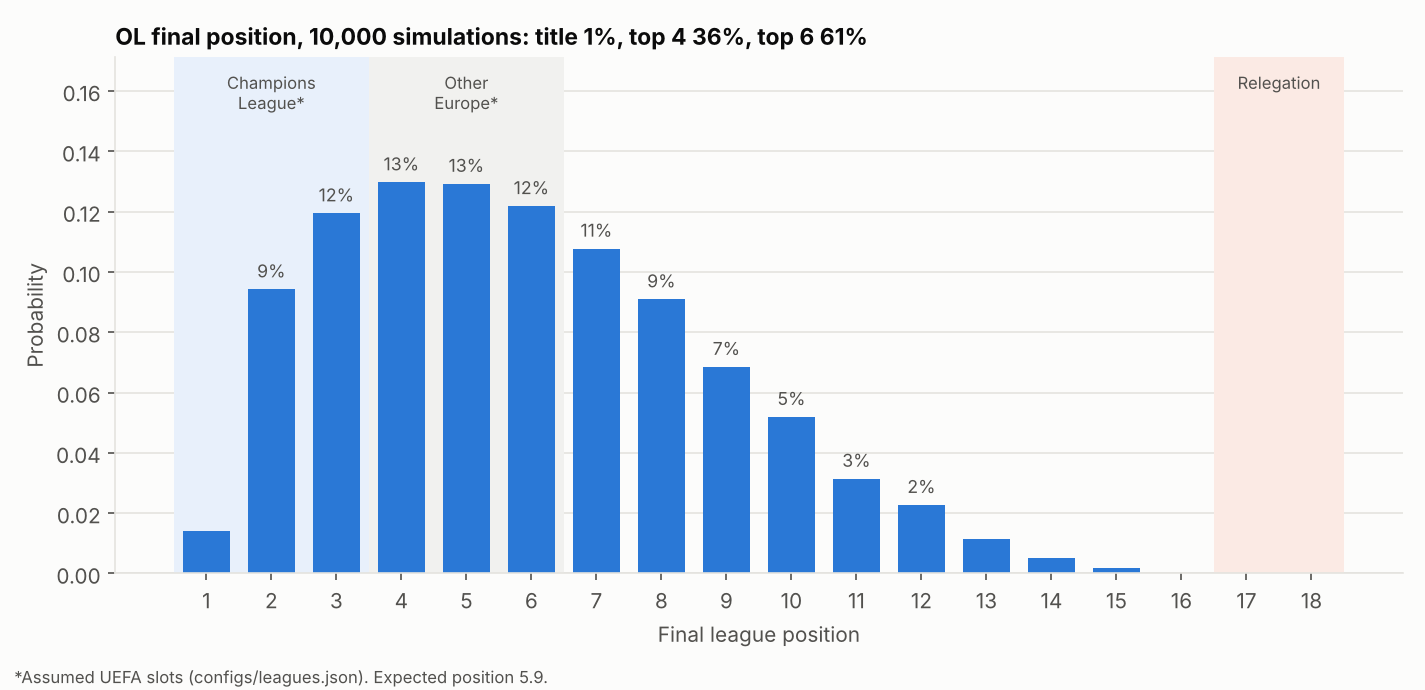
\includegraphics[width=0.8\textwidth]{figures/sim_ol_position.png}\caption{Final position of OL over 10{,}000 simulated seasons.}\label{fig:pos}\end{figure}

The average final position of OL is \textbf{5.9}; the most likely finishes are fourth and fifth (13\% and 13\%), but the distribution is wide:
after 8 matches the clubs from 2nd to 7th place are within 3 points of each other, so the forecast rests on team strength rather than on the table.

\section{Champions League and Europa League}\label{sec:ucl}

The aim is to use the real fixtures and to combine each club's performance in its own championship; OL plays the Europa League this season. The calendars (144 league-phase matches and 36 clubs in each competition) come from Wikipedia;
at the snapshot date 29 Champions League matches and 54 Europa League matches had been recorded there, and the others are simulated.
Domestic leagues are only comparable through matches between their clubs, so I fitted a logistic regression on 3{,}085 past Champions League, Europa League and Conference League matches (2012--2025):

\begin{equation}d^{\text{value}}=\ln V_{\text{home}}-\ln V_{\text{away}},\qquad d^{\text{ppg}}=\mathrm{ppg}_{\text{home}}-\mathrm{ppg}_{\text{away}},\end{equation}
where $\mathrm{ppg}$ is the number of domestic league points per match over the last 20 league matches.

\begin{table}[H]
\caption{European strength model.}
\begin{center}
\small
\begin{tabular}{lc}
\toprule
\textbf{Walk-forward 2023--2025 (943 matches)} & \textbf{Log loss} \\
\midrule
Class frequency & 1.0351 \\
Squad value only & 0.9836 \\
Domestic form only & 1.0368 \\
Value + domestic form & 0.9831 \\
\bottomrule
\end{tabular}
\end{center}
\end{table}

\begin{result}
Squad value carries the signal ($-0.051$ vs the class frequencies, significant). Domestic form adds nothing measurable once value is known ($-0.0005$, 95\% CI $[-0.0048,+0.0038]$).
I keep it because the question asked to combine both, but its weight is small.
\end{result}

I then simulated 20{,}000 times the rest of the league phase, the play-offs (ranks 9--24), the round of 16, quarter-finals, semi-finals and the final (two legs; extra time and penalties close to a coin flip; the final on neutral ground).

\begin{table}[H]
\caption{Champions League 2026/27: probabilities from 20{,}000 simulations.}
\begin{center}
\small
\begin{tabular}{lcccc}
\toprule
\textbf{Club} & \textbf{Top 8} & \textbf{Semi-final} & \textbf{Final} & \textbf{Winner} \\
\midrule
Arsenal & 74\% & 40\% & 24\% & 13.9\% \\
Paris Saint-Germain & 77\% & 41\% & 24\% & 13.6\% \\
Manchester City & 46\% & 37\% & 23\% & 13.1\% \\
Real Madrid & 86\% & 39\% & 23\% & 12.4\% \\
Barcelona & 59\% & 37\% & 22\% & 12.1\% \\
Bayern Munich & 66\% & 34\% & 18\% & 9.9\% \\
Liverpool & 70\% & 27\% & 13\% & 5.6\% \\
Inter Milan & 27\% & 16\% & 7\% & 3.1\% \\
Manchester United & 18\% & 14\% & 6\% & 2.7\% \\
Sporting CP & 27\% & 12\% & 5\% & 1.7\% \\
\bottomrule
\end{tabular}
\end{center}
\end{table}

\begin{table}[H]
\caption{Europa League 2026/27: probabilities from 20{,}000 simulations (OL included).}
\begin{center}
\small
\begin{tabular}{lcccc}
\toprule
\textbf{Club} & \textbf{Top 8} & \textbf{Semi-final} & \textbf{Final} & \textbf{Winner} \\
\midrule
Bournemouth & 97\% & 43\% & 26\% & 15.2\% \\
Juventus & 89\% & 42\% & 25\% & 14.2\% \\
Benfica & 96\% & 38\% & 21\% & 11.2\% \\
Bayer Leverkusen & 82\% & 36\% & 20\% & 10.7\% \\
Crystal Palace & 35\% & 30\% & 16\% & 8.9\% \\
Milan & 31\% & 29\% & 16\% & 8.5\% \\
Sunderland & 70\% & 28\% & 14\% & 6.7\% \\
Rennes & 46\% & 23\% & 11\% & 4.8\% \\
\textbf{Lyon} & \textbf{42\%} & \textbf{20\%} & \textbf{9\%} & \textbf{4.0\%} \\
Marseille & 1\% & 12\% & 6\% & 2.8\% \\
\bottomrule
\end{tabular}
\end{center}
\end{table}

There is \textbf{no clear favourite} in either competition. In the Champions League 3 clubs are within one point of the leader (Arsenal, Paris Saint-Germain, Manchester City), the best at 13.9\%;
in the Europa League the leader, Bournemouth, has 15.2\%, followed by Juventus (14.2\%) and Benfica (11.2\%), and OL has 4.0\%.
These models are validated match by match, not on whole tournaments; the knockout bracket is approximate; 3 Champions League clubs and 8 Europa League clubs are not in the squad-value data and are assumed weak.

\section{Limitations}

\begin{itemize}
\item No injuries, suspensions, line-ups or coaching news (the likely reason the bookmaker is better); no real xG.
\item Squad values are a crowd-sourced snapshot (June 2026); 13 clubs have no value.
\item The bookmaker benchmark uses Bet365 pre-match prices with a simple margin removal.
\item Few validation windows; the SVM is under-tuned; online updating was tested for the linear model only.
\item Simulation: intervals are too narrow in the backtest, UEFA places are assumptions, and strength is constant apart from a random shock.
\item Wikipedia lags: 25 Champions League matches played before the snapshot are not recorded there yet, and are simulated.
\end{itemize}

\section{Conclusion}

On public data, football results can be forecast with \emph{well-calibrated probabilities that are only modestly sharper than team strength alone}. Elo and squad value explain most of what is predictable.
The chosen model, a regularised multinomial logistic regression, is as good as boosting and neural networks: complexity did not pay. The models cannot beat the betting market and add no information to it,
which is consistent with an efficient market. For OL, the model sees the fifth most valuable squad of Ligue 1 and a middling start: about 54.6 points, an average finish of 5.9 and a 23\% chance of a Champions League place.
So the disclaimer at the beginning stands: I really hope the ML is wrong.

\textbf{Reproducibility.} Code, tests (including the leakage test) and the interactive website are in the repository; \texttt{make weekly} refreshes the data, the variables, the OL predictions, the simulations and the website. All numbers come from \texttt{reports/tables/}.
\begin{thebibliography}{9}\small
\bibitem{brier1950} G.~W. Brier. Verification of forecasts expressed in terms of probability. \emph{Monthly Weather Review}, 78(1):1--3, 1950.
\bibitem{gneiting2007} T.~Gneiting and A.~E. Raftery. Strictly proper scoring rules, prediction, and estimation. \emph{Journal of the American Statistical Association}, 102(477):359--378, 2007.
\bibitem{pedregosa2011} F.~Pedregosa et al. Scikit-learn: machine learning in Python. \emph{Journal of Machine Learning Research}, 12:2825--2830, 2011.
\bibitem{elo1978} A.~E. Elo. \emph{The Rating of Chessplayers, Past and Present}. Arco, 1978.
\bibitem{dixon1997} M.~J. Dixon and S.~G. Coles. Modelling association football scores and inefficiencies in the football betting market. \emph{Journal of the Royal Statistical Society C}, 46(2):265--280, 1997.
\end{thebibliography}

\end{document}
